\section{Daylight Factor Calculation}\label{daylight-factor-calculation}

The daylighting factor calculation using the SplitFlux daylighting method is described below.

% table 25
\begin{longtable}[c]{p{1.25in}p{2.0in}p{1.25in}p{1.5in}}

\caption{Variables in Daylighting Calculations \label{table:variables-in-daylighting-calculations}} \tabularnewline
\toprule 
Mathematical Variable & Description & Units & Internal Variable \tabularnewline
\midrule
\endfirsthead

\caption[]{Variables in Daylighting Calculations} \tabularnewline
\toprule 
Mathematical Variable & Description & Units & Internal Variable \tabularnewline
\midrule
\endhead

$E_{h,\text{sky}}$ & Exterior horizontal illuminance due to light from the sky & lux & GILSK \tabularnewline
$E_{h,\text{sun}}$ & Exterior horizontal illuminance due to light from the sun & lux & GILSU \tabularnewline
$d_{\text{sky}}$, $d_{\text{sun}}$ & Interior illuminance factor due to sky, sun related light & --- & DFACSK,DFACSU \tabularnewline
$w_{\text{sky}}$, $w_{\text{sun}}$ & Window luminance factor due to sky, sun related light & cd/lm & SFACSK, SFACSU \tabularnewline
$b_{\text{sky}}$, $b_{\text{sun}}$ & Window background luminance factor due to sky, sun related light & cd/lm & BFACSK, BFACSU \tabularnewline
$N$ & Number of exterior windows in a zone & --- & NWD \tabularnewline
$\theta_{\text{sky}}$, $\varphi_{\text{sky}}$ & Azimuth and altitude angles of a point in the sky & radians & THSKY, PHSKY \tabularnewline
$\Psi_{cs}$ & Clear sky luminance distribution & $cd/m^2$ & --- \tabularnewline
$\Psi_{ts}$ & Clear turbid sky luminance distribution & $cd/m^2$ & --- \tabularnewline
$\Psi_{is}$ & Intermediate sky luminance distribution & $cd/m^2$ & --- \tabularnewline
$\Psi_{os}$ & Overcast sky luminance distribution & $cd/m^2$ & --- \tabularnewline
$\varphi_{\text{sun}}$ & Altitude angle of the sun & radians or degrees & PHSUN \tabularnewline
$\gamma$ & Angle between point in the sky and the sun; or angle between vertical and ray from reference point to window element & radians & G \tabularnewline
$L_z$ & Sky zenith luminance & cd/m2 & ZENL \tabularnewline
$m$ & Optical air mass of the atmosphere & m & AM \tabularnewline
$h$ & Building altitude & m & ELEVATION \tabularnewline
$E_{h,k}$ & Exterior horizontal illuminance for sky type k & lux & --- \tabularnewline
$N_{\theta}$, $N_{\varphi}$ & Number of azimuth, altitude steps for sky integration & --- & NTH, NPH \tabularnewline
$\vec{R}_{ref}$ & Vector from zone origin to reference point & m & RREF \tabularnewline
$\vec{R}_{win}$ & Vector from zone origin to window element & m & RWIN \tabularnewline
$\mathrm{d}\Omega$ & Solid angle subtended by window element & steradians & DOMEGA \tabularnewline
$L_w$ & Luminance of a window element as seen from reference point & $cd/m^2$ & WLUMSK, WLUMSU \tabularnewline
$L_{w,\text{shade}}$ & Luminance of window element with shade in place & $cd/m^2$ & WLUMSK, WLUMSU \tabularnewline
$\mathrm{d}E_h$ & Horizontal illuminance at reference point from window element & lux & --- \tabularnewline
$\mathrm{d}x$, $\mathrm{d}y$ & Size of window element & m & DWX, DWY \tabularnewline
$D$ & Distance from reference point to window element & m & DIS \tabularnewline
$B$ & Angle between window element's outward normal and ray from reference point to window element & radians & --- \tabularnewline
$\hat{R}_{ray}$ & Unit vector from reference point to window element & --- & RAY \tabularnewline
$\hat{W}_{n}$ & Unit vector normal to window element, pointing away from zone & --- & WNORM \tabularnewline
$\hat{W}_{21}$ & Unit vector along window y-axis & --- & W21 \tabularnewline
$\hat{W}_{23}$ & Unit vector along window x-axis & --- & W23 \tabularnewline
$\tau_{\text{vis}}$ & Glass visible transmittance & --- & TVISB \tabularnewline
$L$ & Luminance of sky or obstruction & $cd/m^2$ & ELUM, --- \tabularnewline
$\phi_{FW}$ & Downgoing luminous flux from a window & lm & FLFW --- \tabularnewline
$\phi_{CW}$ & Upgoing luminous flux from a window & lm & FLCW --- \tabularnewline
$F_1$ & First-reflected flux & lm & - \tabularnewline
$\rho_{FW}$ & Area-weighted reflectance of floor and upper part of walls & --- & SurfaceWindow\%RhoFloorWall \tabularnewline
$\rho_{CW}$ & Area-weighted reflectance of ceiling and upper part of walls & --- & SurfaceWindow\%RhoCeilingWall \tabularnewline
$E_r$ & Average internally-reflected illuminance & lux & EINTSK, EINTSU \tabularnewline
$A$ & Total inside surface area of a zone & $m^2$ & ATOT \tabularnewline
$\rho$ & Area-weighted average reflectance of zone interior surfaces & --- & ZoneDaylight\%AveVisDiffREflect \tabularnewline
$\theta$, $\varphi$ & Azimuth and altitude angle of a sky or ground element & radians & TH, PH \tabularnewline
$L(\theta, \varphi)$ & Luminance of sky or ground element at $(\theta, \varphi)$ & $cd/m^2$ & HitPointLum-- \tabularnewline
$A_w$ & Area of glazed part of window & $m^2$ & Surface\%Area \tabularnewline
$\beta$ & Angle of incidence, at center of window, of light from a sky or ground element & radians & --- \tabularnewline
$T(\beta)$ & Glazing visible transmittance at incidence angle $\beta$ & --- & TVISBR \tabularnewline
$\mathrm{d}\phi_{inc}$ & Luminous flux incident on window from sky or ground element & lm & --- \tabularnewline
$\mathrm{d}\phi$ & Luminous flux from sky or ground element transmitted through window & lm & --- \tabularnewline
$\mathrm{d}\phi_{FW}$, $\mathrm{d}\phi_{CW}$ & Luminous flux from sky or ground element transmitted through window and going downward, upward & lm & - \tabularnewline
$\theta_{\text{min}}$, $\theta_{\text{max}}$ & Azimuth angle integration limits & radians & THMIN, THMAX \tabularnewline
$\varphi_w$ & Window normal altitude angle & radians & - \tabularnewline
$\phi_{sh}$, $\phi_{unsh}$ & Transmitted flux through window and shade, without shade & lm & --- \tabularnewline
$\phi_{CW,sh}$, $\phi_{FW,sh}$ & Upgoing and downgoing portions of transmitted flux through window with shade & lm & --- \tabularnewline
$\phi_{CW,unsh}$, $\phi_{FW,unsh}$ & Upgoing and downgoing portions of transmitted flux through window without shade & lm & --- \tabularnewline
$f$ & Fraction of hemisphere seen by the inside of window that lies above the window midplane & --- & SurfaceWindow\%Fraction UpGoing \tabularnewline
$\phi_{inc}$ & Flux incident on glazing from direct sun & lm & --- \tabularnewline
$f_{\text{sunlit}}$ & Fraction of glazing that is sunlit & --- & SunLitFrac \tabularnewline
$\phi$ & Transmitted flux from direct sun & --- & --- \tabularnewline
$L_{sh}$ & Luminance of window with shade & $cd/m^2$ & --- \tabularnewline
$L_b$ & Window background luminance & $cd/m^2$ & BLUM \tabularnewline
$G$ & Discomfort glare constant & --- & GTOT \tabularnewline
$G_i$ & Discomfort glare constant from window $i$ & --- & --- \tabularnewline
$\omega$ & Solid angle subtended by window with respect to reference point & steradians & SolidAngAtRefPt \tabularnewline
$\Omega$ & Solid angle subtended by window with respect to reference point, modified to take direction of occupant view into account & steradians & SolidAngAtRefPtWtd \tabularnewline
$N_x$, $N_y$ & Number of elements in $x$ and $y$ direction that window is divided into for glare calculation & --- & NWX, NWY \tabularnewline
$p(x_R, y_R)$ & Position factor for horizontal and vertical displacement ratios $x_R$ and $y_R$ & --- & DayltgGlarePositionFactor \tabularnewline
$p_H$ & Hopkinson position factor & --- & DayltgGlarePositionFactor \tabularnewline
$L_b$ & Window background luminance & $cd/m^2$ & BLUM \tabularnewline
$E_b$ & Illuminance on window background & lm & --- \tabularnewline
$E_r$ & Total internally-reflected component of daylight illuminance & lm & --- \tabularnewline
$E_s$ & Illuminance setpoint & lm & IllumSetPoint \tabularnewline
$G_I$ & Glare Index & --- & GLINDX \tabularnewline
\bottomrule
\end{longtable}

\subsection{Overview}\label{overview-013}

There are three types of daylight factors: interior illuminance factors, window luminance factors, and window background luminance factors. To calculate these factors the following steps are carried out for each hourly sun position on the sun paths for the design days and for representative days\footnote{The sun positions for which the daylight factors are calculated are the same as those for which the solar shadowing calculations are done.} during the simulation run period:

1.~~~~Calculate exterior horizontal daylight illuminance from sky and sun for standard (CIE) clear and overcast skies.

2.~~~~Calculate interior illuminance, window luminance and window background luminance for each window/reference-point combination, for bare and for shaded window conditions (if a shading device has been specified), for overcast sky and for standard clear sky.

3.~~~~Divide by exterior horizontal illuminance to obtain daylight factors.

\subsection{Interior Illuminance Components}\label{interior-illuminance-components}

To calculate daylight factors, daylight incident on a window is separated into two components: (1) light that originates from the \emph{sky} and reaches the window directly or by reflection from exterior surfaces; and (2) light that originates from the \emph{sun} and reaches the window directly or by reflection from exterior surfaces. Light from the window reaches the workplane directly or via reflection from the interior surfaces of the room.

For fixed sun position, sky condition (clear or overcast) and room geometry, the sky-related interior daylight will be proportional to the exterior horizontal illuminance, \emph{E\(_{h,sky}\)}, due to light from the sky. Similarly, the sun-related interior daylight will be proportional to the exterior horizontal solar illuminance, \emph{E\(_{h,sun}\)}.

\subsection{Daylight Factors}\label{daylight-factors}

The following daylight factors are calculated:

\begin{equation}
{d_{sky}} = \frac{{{\rm{Illuminance~at~reference~point~due~to~sky-related~light}}}}{{{E_{h,sky}}}}
\end{equation}

\begin{equation}
{d_{sun}} = \frac{{{\rm{Illuminance~at~reference~point~due~to~sun-related~light}}}}{{{E_{h,sun}}}}
\end{equation}

\begin{equation}
{w_{sky}} = \frac{{{\rm{Average~window~luminance~due~to~sky-related~light}}}}{{{E_{h,sky}}}}
\end{equation}

\begin{equation}
{w_{sun}} = \frac{{{\rm{Average~window~luminance~due~to~sun-related~light}}}}{{{E_{h,sun}}}}
\end{equation}

\begin{equation}
{b_{sky}} = \frac{{{\rm{Window~background~luminance~due~to~sky-related~light}}}}{{{E_{h,sky}}}}
\end{equation}

\begin{equation}
{b_{sun}} = \frac{{{\rm{Window~background~luminance~due~to~sun-related~light}}}}{{{E_{h,sun}}}}
\end{equation}

For a daylit zone with \emph{N} windows these six daylight factors are calculated for each of the following combinations of reference point, window, sky-condition/sun-position and shading device:

\begin{equation}
\left[
    \begin{array}{c}
      Ref~pt~1 \\
      Ref~pt~2
    \end{array}
  \right]
  \left[
    \begin{array}{c}
      Window~1 \\
      Window~2 \\
      ... \\
      Window~N
    \end{array}
  \right]
  \left[
    \begin{array}{c}
      Clear~sky,~first~sun-up~hour \\
      Clear/turbid~sky,~first~sun-up~hour \\
      Intermediate~sky,~first~sun-up~hour \\
      Overcast~sky,~first~sun-up~hour \\
      ... \\
      Clear~sky,~last~sun-up~hour \\
      Clear/turbid~sky,~last~sun-up~hour \\
      Intermediate~sky,~last~sun-up~hour \\
      Overcase~sky,~last~sun-up~hour
    \end{array}
   \right]
   \left[
     \begin{array}{c}
       Unshaded~window \\
       Shaded~window \\
       (if~shade~assigned)
     \end{array}
   \right]
\end{equation}

\subsection{Sky Luminance Distributions}\label{sky-luminance-distributions}

The luminance distribution of the sky is represented as a superposition of four standard CIE skies using the approach described in (Perez et al. 1990). The standard skies are as follows.

\subsubsection{Clear Sky}\label{clear-sky}

The clear sky luminance distribution has the form (Kittler, 1965; CIE, 1973)

\begin{equation}
{\psi_{cs}}({\theta_{sky}},{\phi_{sky}}) = {L_z}\frac{{(0.91 + 10{e^{ - 3\gamma }} + 0.45{{\cos }^2}\gamma )(1 - {e^{ - 0.32{\rm{cosec}}{\phi_{sky}}}})}}{{0.27385(0.91 + 10{e^{ - 3(\frac{\pi }{2} - {\phi_{sun}})}} + 0.45{{\sin }^2}{\phi_{sun}})}}
\end{equation}

Here, \emph{L\(_{z}\)} is the zenith luminance (i.e., the luminance of the sky at a point directly overhead). In the calculation of daylight factors, which are ratios of interior and exterior illumination quantities that are both proportional to \emph{L\(_{z}\)}, the zenith luminance cancels out. For this reason we will use \emph{L\(_{z}\)} = 1.0 for all sky luminance distributions.

The various angles, which are defined in the building coordinate system, are shown in Figure~\ref{fig:angles-appearing-in-the-expression-for}. The angle, $\gamma$, between sun and sky element is given by:

\begin{equation}
\gamma  = {\cos ^{ - 1}}\left[ {\sin {\phi_{sky}}\sin {\phi_{sun}} + \cos {\phi_{sky}}\cos {\phi_{sun}}\cos ({\theta_{sky}} - {\theta_{sun}})} \right]
\end{equation}

The general characteristics of the clear-sky luminance distribution are a large peak near the sun; a minimum at a point on the other side of~ the zenith from the sun, in the vertical plane containing the sun; and an increase in luminance as the horizon is approached.

\subsubsection{Clear Turbid Sky}\label{clear-turbid-sky}

The clear turbid sky luminance distribution has the form {[}Matsuura, 1987{]}:

\begin{equation}
{\psi_{ts}}({\theta_{sky}},{\phi_{sky}}) = {L_z}\frac{{(0.856 + 16{e^{ - 3\gamma }} + 0.3{{\cos }^2}\gamma )(1 - {e^{ - 0.32{\rm{cosec}}{\phi_{sky}}}})}}{{0.27385(0.856 + 10{e^{ - 3(\frac{\pi }{2} - {\phi_{sun}})}} + 0.3{{\sin }^2}{\phi_{sun}})}}
\end{equation}

\subsubsection{Intermediate Sky}\label{intermediate-sky}

The intermediate sky luminance distribution has the form {[}Matsuura, 1987{]}:

\begin{equation}
{\psi_{is}}\left( {{\theta_{sky}},{\phi_{sky}}} \right) = {L_z}{Z_1}{Z_2}/({Z_3}{Z_4})
\end{equation}

where

\begin{equation}
{Z_1} = \left[ {1.35(\sin (3.59{\phi_{sky}} - 0.009) + 2.31)\sin (2.6{\phi_{sun}} + 0.316) + {\phi_{sky}} + 4.799} \right]/2.326 
\end{equation}

\begin{equation}
{Z_2} = \exp \left[ { - 0.563\gamma \{ ({\phi_{sun}} - 0.008)({\phi_{sky}} + 1.059) + 0.812\} } \right]
\end{equation}

\begin{equation}
{Z_3} = 0.99224\sin (2.6{\phi_{sun}} + 0.316) + 2.73852
\end{equation}

\begin{equation}
{Z_4} = \exp \left[ { - 0.563({\frac{\pi}{2}} - {\phi_{sun}})\{ 2.6298({\phi_{sun}} - 0.008) + 0.812\} } \right]
\end{equation}

\begin{figure}[hbtp] % fig 57
\centering
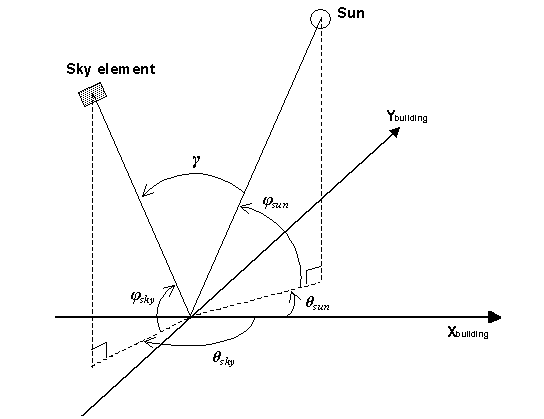
\includegraphics[width=0.9\textwidth, height=0.9\textheight, keepaspectratio=true]{media/image733.png}
\caption{Angles appearing in the expression for the clear-sky luminance distribution. \protect \label{fig:angles-appearing-in-the-expression-for}}
\end{figure}

\subsubsection{Overcast Sky}\label{overcast-sky}

The overcast sky luminance distribution has the form {[}Moon \& Spencer, 1942{]}:

\begin{equation}
{\psi_{os}}({\phi_{sky}}) = {L_z}\frac{{1 + 2\sin {\phi_{sky}}}}{3}
\end{equation}

Unlike the clear sky case, the overcast sky distribution does not depend on the solar azimuth or the sky azimuth. Note that at fixed solar altitude the zenith (\({\phi_{sky}} = \pi /2\) ) is three times brighter than the horizon (\({\phi_{sky}} = 0\) ).

\subsection{Direct Normal Solar Illuminance}\label{direct-normal-solar-illuminance}

For purposes of calculating daylight factors associated with beam solar illuminance, the direct normal solar illuminance is taken to be 1.0 W/m\(^{2}\). The actual direct normal solar illuminance, determined from direct normal solar irradiance from the weather file and empirically-determined luminous efficacy, is used in the time-step calculation.

\subsection{Exterior Horizontal Illuminance}\label{exterior-horizontal-illuminance}

The illuminance on an unobstructed horizontal plane due to diffuse radiation from the sky is calculated for each of the four sky types by integrating over the appropriate sky luminance distribution:

\begin{equation}
{E_{h,k}} = \int\limits_0^{2\pi } {\int\limits_0^{\pi /2} {{\psi_k}({\theta_{sky}},{\phi_{sky}})\sin {\phi_{sky}}\cos {\phi_{sky}}d{\theta_{sky}}} } d{\phi_{sky}}
\end{equation}

where \emph{k} = \emph{cs}, \emph{ts}, \emph{is} or \emph{os}. The integral is evaluated as a double summation:

\begin{equation}
{E_{h,k}} = \sum\limits_{i = 1}^{{N_\theta }} {\sum\limits_{j = 1}^{{N_\phi }} {{\psi_k}\left( {{\theta_{sky}}(i),{\phi_{sky}}(j)} \right)} } \sin {\phi_{sky}}(j)\cos {\phi_{sky}}(j)\Delta {\theta_{sky}}\Delta {\phi_{sky}}
\end{equation}

where

\begin{equation}
\begin{array}{l}
    \theta_{sky}(i) = (i - 1/2) \Delta \theta_{sky} \\
    \phi_{sky}(j) = (j - 1/2) \Delta \phi_{sky} \\
    \Delta \theta_{sky} = 2 \pi / N_{\theta} \\
    \Delta \phi_{sky} = \pi / 2N_{\phi} 
\end{array}
\end{equation}

\({N_\theta } = 18\) ~and \({N_\phi } = 8\) ~were found to give a \(\pm 1\%\) accuracy in the calculation of \({E_h}_{,k}\).

\subsection{Direct Component of Interior Daylight Illuminance}\label{direct-component-of-interior-daylight-illuminance}

The direct daylight illuminance at a reference point from a particular window is determined by dividing the window into an x-y grid and finding the flux reaching the reference point from each grid element. The geometry involved is shown in Figure~\ref{fig:geometry-for-calculation-of-direct-component}. The horizontal illuminance at the reference point, \({\vec R_{ref}}\) , due to a window element is:

\begin{equation}
d{E_h} = {L_w}d\Omega \cos \gamma
\end{equation}

where \emph{L\(_{w}\)} is the luminance of the window element as seen from the reference point.

The subtended solid angle is approximated by:

\begin{equation}
d\Omega  = \frac{{dxdy}}{{{D^2}}}\cos B
\label{eq:SubtendedSolidAngle}
\end{equation}

where

\begin{equation}
D = \left| {{{\bar R}_{win}} - {{\bar R}_{ref}}} \right|
\end{equation}

\emph{CosB} is found from:

\begin{equation}
\cos B = {\hat R_{ray}} \cdot {\hat W_n}
\end{equation}

where

\begin{equation}
{\vec R_{ray}} = ({\vec R_{win}} - {\vec R_{ref}})/D
\end{equation}

\begin{equation}
{\hat W_n} = {\rm{ window~outward~normal }} = {\hat W_{21}} \times {\hat W_{23}} = \frac{{{{\vec W}_1} - {{\vec W}_2}}}{{\left| {{{\vec W}_1} - {{\vec W}_2}} \right|}} \times \frac{{{{\vec W}_3} - {{\vec W}_2}}}{{\left| {{{\vec W}_3} - {{\vec W}_2}} \right|}}
\end{equation}

Equation~\ref{eq:SubtendedSolidAngle} becomes exact as \(dx/D\) and \(dy/D \to 0\) and is accurate to better than about 1\% for \(dx \le D/4\) and \(dy \le D/4\) .

The net illuminance from the window is obtained by summing the contributions from all the window elements:

\begin{equation}
{E_h} = \sum\limits_{\scriptstyle \substack{window \\ elements}} {{L_w}d\Omega \cos \gamma }
\label{eq:NetIlluminanceFromWindow}
\end{equation}

In performing the summation, window elements that lie below the workplane (\(\cos \gamma < 0\) ) are omitted since light from these elements cannot reach the workplane directly.

\begin{figure}[hbtp] % fig 58
\centering

\includegraphics[width=0.9\textwidth, height=0.9\textheight, keepaspectratio=true]{media/image755.png}
\caption{Geometry for calculation of direct component of daylight illuminance at a reference point. Vectors R\(_ref\), W\(_1\), W\(_2\), W\(_3\) and R\(_win\) are in the building coordinate system. \protect \label{fig:geometry-for-calculation-of-direct-component}}
\end{figure}

\subsubsection{Unshaded Window}\label{unshaded-window}

For the unshaded window case, the luminance of the window element is found by projecting the ray from reference point to window element and determining whether it intersects the sky or an exterior obstruction such as an overhang. If \emph{L} is the corresponding luminance of the sky or obstruction, the window luminance is:

\begin{equation}
{L_w} = L{\tau_{vis}}cosB
\end{equation}

where \({\tau_{vis}}\) is the visible transmittance of the glass for incidence angle \emph{B}.

Exterior obstructions are generally opaque (like fins, overhangs, neighboring buildings, and the building's own wall and roof surfaces) but can be transmitting (like a tree or translucent awning). Exterior obstructions are assumed to be non-reflecting. If \emph{L\(_{sky}\)} is the sky luminance and \emph{$\tau$\(_{obs}\)} is the transmittance of the obstruction (assumed independent of incidence angle), then \(L = L_{sky} \tau_{obs}\). Interior obstructions are assumed to be opaque ($\tau$\(_{obs}\) = 0).

\subsubsection{Shaded Window}\label{shaded-window}

For the window-plus-shade case the shade is assumed to be a perfect diffuser, i.e., the luminance of the shade is independent of angle of emission of light, position on shade, and angle of incidence of solar radiation falling on the shade. Closely-woven drapery fabric and translucent roller shades are closer to being perfect diffusers than Venetian blinds or other slatted devices, which usually have non-uniform luminance characteristics.

The calculation of the window luminance with the shade in place, \emph{L\(_{w,sh}\)}, is described in {[}Winkelmann, 1983{]}. The illuminance contribution at the reference point from a shaded window element is then given by Equation~\ref{eq:NetIlluminanceFromWindow} with \({L_w} = {L_{w,sh}}\) .

\subsection{Internally-Reflected Component of Interior Daylight Illuminance}\label{internally-reflected-component-of-interior-daylight-illuminance}

Daylight reaching a reference point after reflection from interior surfaces is calculated using the \emph{split-flux} method {[}Hopkinson et al., 1954{]}, {[}Lynes, 1968{]}. In this method the daylight transmitted by the window is split into two parts---a downward-going flux, \({\Phi_{FW}}\) (lumens), which falls on the floor and portions of the walls below the imaginary horizontal plane passing through the center of the window (\emph{window midplane}), and an upward-going flux, \({\Phi_{CW}}\) , that strikes the ceiling and portions of the walls above the window midplane. A fraction of these fluxes is absorbed by the room surfaces. The remainder, the first-reflected flux, \emph{F\(_{1}\)}, is approximated by

\begin{equation}
{F_1} = {\Phi_{FW}}{\rho_{FW}} + {\Phi_{CW}}{\rho_{CW}}
\end{equation}

where \emph{$\rho$\(_{FW}\)} is the area-weighted average reflectance of the floor and those parts of the walls below the window midplane, and \emph{$\rho$\(_{CW}\)} is the area-weighted average reflectance of the ceiling and those parts of the walls above the window midplane.

To find the final average internally-reflected illuminance, \emph{E\(_{r}\)}, on the room surfaces (which in this method is uniform throughout the room) a flux balance is used. The total reflected flux absorbed by the room surfaces (or lost through the windows) is \emph{AE\(_{r}\)(1-$\rho$)}, where \emph{A} is the total inside surface area of the floor, walls, ceiling and windows in the room, and \emph{$\rho$} is the area-weighted average reflectance of the room surfaces, including windows. From conservation of energy:

\begin{equation}
A{E_r}(1 - \rho ) = {F_1}
\end{equation}

or

\begin{equation}
{E_r} = \frac{{{\Phi_{FW}}{\rho_{FW}} + {\Phi_{CW}}{\rho_{CW}}}}{{A(1 - \rho )}}
\end{equation}

This procedure assumes that the room behaves like an integrating sphere with perfectly diffusing interior surfaces and with no internal obstructions. It therefore works best for rooms that are close to cubical in shape, have matte surfaces (which is usually the case), and have no internal partitions. Deviations from these conditions, such as would be the case for rooms whose depth measured from the window-wall is more than three times greater than ceiling height, can lead to substantial inaccuracies in the split-flux calculation.

\subsection{Transmitted Flux from Sky and Ground}\label{transmitted-flux-from-sky-and-ground}

The luminous flux incident on the center of the window from a luminous element of sky or ground at angular position \((\theta ,\phi )\), of luminance \(L(\theta ,\phi )\), and subtending a solid angle \(\cos \phi d\theta d\phi\)~is:

\begin{equation}
d{\Phi_{inc}} = {A_w}L(\theta ,\phi )\cos \beta \cos \phi d\theta d\phi
\end{equation}

The transmitted flux is:

\begin{equation}
d\Phi  = d{\Phi_{inc}}T(\beta )
\end{equation}

where \emph{T($\beta$)} is the window transmittance for light at incidence angle \emph{$\beta$}. This transmittance depends on whether or not the window has a shade.

For an unshaded window the total downgoing transmitted flux is obtained by integrating over the part of the exterior hemisphere seen by the window that lies above the window midplane. This gives:

\begin{equation}
{\Phi_{FW,unshaded}} = {A_w}\int\limits_{{\theta_{\min }}}^{{\theta_{\max }}} {\int\limits_0^{\pi /2} {L(\theta ,\phi )T(\beta )\cos \beta \cos \phi d\theta d\phi } }
\label{eq:PhiFWUnshaded}
\end{equation}

The upgoing flux is obtained similarly by integrating over the part of the exterior hemisphere that lies below the window midplane:

\begin{equation}
{\Phi_{CW,unshaded}} = {A_w}\int\limits_{{\theta_{\min }}}^{{\theta_{\max }}} {\int\limits_{\pi /2 - {\phi_w}}^0 {L(\theta ,\phi )T(\beta )\cos \beta \cos \phi d\theta d\phi } }
\label{eq:PhiCWUnshaded}
\end{equation}

where \({\phi_w}\) is the angle the window outward normal makes with the horizontal plane.

For a window with a diffusing shade the total transmitted flux is:

\begin{equation}
{\Phi_{sh}} = {A_w}\int\limits_{{\theta_{\min }}}^{{\theta_{\max }}} {\int\limits_{\pi /2 - {\phi_w}}^{\pi /2} {L(\theta ,\phi )T(\beta )\cos \beta \cos \phi d\theta d\phi } }
\label{eq:PhiSh}
\end{equation}

The downgoing and upgoing portions of this flux are:

\begin{equation}
\begin{array}{l}
    \Phi_{FW,sh} = \Phi (1 - f) \\
    \Phi_{CW,sh} = \Phi f
\end{array}
\end{equation}

where \emph{f}, the fraction of the hemisphere seen by the inside of the window that lies above the window midplane, is given by

\begin{equation}
f = 0.5 - {\phi_w}/\pi
\end{equation}

For a vertical window (\({\phi_w} = 0\)) the up- and down-going transmitted fluxes are equal:

\begin{equation}
{\Phi_{FW,sh}} = {\Phi_{CW,sh}} = \Phi /2
\end{equation}

For a horizontal skylight (\({\phi_w} = \pi /2\)):

\begin{equation}
{\Phi_{FW,sh}} = \Phi ,{\Phi_{CW,sh}} = 0
\end{equation}

The limits of integration of \({\theta}\) in Equations~\ref{eq:PhiFWUnshaded},~\ref{eq:PhiCWUnshaded} and~\ref{eq:PhiSh} depend on \(\phi\) . From Figure 12 of Winkelmann (1983), we have:

\begin{equation}
\sin \alpha  = \sin (A - \pi /2) = \frac{{\sin \phi \tan {\phi_w}}}{{\cos \phi }}
\end{equation}

which gives:

\begin{equation}
A = {\cos ^{ - 1}}(\tan \phi \tan {\phi_w})
\end{equation}

Thus:

\begin{equation}
\begin{array}{rl}
    \theta_{min} & =  - \left| \cos^{-1}(-\tan\phi\tan\phi_w) \right| \\
    \theta_{max} & = \left| \cos^{-1}(-\tan\phi\tan\phi_w) \right| 
\end{array}
\end{equation}

\subsection{Transmitted Flux from Direct Sun}\label{transmitted-flux-from-direct-sun}

The flux incident on the window from direct sun is:

\begin{equation}
{\Phi_{inc}} = {A_w}{E_{DN}}\cos \beta {f_{sunlit}}
\end{equation}

The transmitted flux is:

\begin{equation}
\Phi  = T(\beta ){\Phi_{inc}}
\end{equation}

where T is the net transmittance of the window glazing (plus shade, if present).

For an unshaded window all of the transmitted flux is downward since the sun always lies above the window midplane. Therefore:

\begin{equation}
\begin{array}{l}
    \Phi_{FW,unsh} = \Phi \\
    \Phi_{CW,unsh} = 0
\end{array}
\end{equation}

For a window with a diffusing shade:

\begin{equation}
  \begin{array}{rl}
    \Phi_{FW,sh} &= \Phi (1 - f) \\
    \Phi_{CW,sh} &= \Phi f
  \end{array}
\end{equation}

\subsection{Luminance of Shaded Window}\label{luminance-of-shaded-window}

The luminance of a shaded window is determined at the same time that the transmitted flux is calculated. It is given by:

\begin{equation}
{L_{sh}} = \frac{1}{\pi }\int\limits_{{\theta_{\min }}}^{{\theta_{\max }}} {\int\limits_{\pi /2 - {\phi_w}}^{\pi /2} {L(\theta ,\phi )T(\beta )\cos \beta \cos \phi d\theta d\phi } }
\end{equation}

\subsection{Daylight Discomfort Glare}\label{daylight-discomfort-glare}

The discomfort glare at a reference point due to luminance contrast between a window and the interior surfaces surrounding the window is given by {[}Hopkinson, 1970{]} and {[}Hopkinson, 1972{]}:

\begin{equation}
G = \frac{{L_w^{1.6}{\Omega ^{0.8}}}}{{{L_b} + 0.07{\omega ^{0.5}}{L_w}}}
\end{equation}

where

\emph{G} = discomfort glare constant

\emph{L\(_{w}\)} = average luminance of the window as seen from the reference point

\emph{Ω} = solid angle subtended by window, modified to take direction of occupant view into account

\emph{L\(_{b}\)} = luminance of the background area surrounding the window

By dividing the window into \emph{N\(_{x}\)} by \emph{N\(_{y}\)} rectangular elements, as is done for calculating the direct component of interior illuminance, we have:

\begin{equation}
{L_w} = \frac{{\sum\limits_{j = 1}^{{N_y}} {\sum\limits_{i = 1}^{{N_x}} {{L_w}(i,j)} } }}{{{N_x}{N_y}}}
\end{equation}

where \emph{L\(_{w}\)(i,j)} is the luminance of element \emph{(i,j)} as seen from the reference point.

Similarly,

\begin{equation}
\omega  = \sum\limits_{j = 1}^{{N_y}} {\sum\limits_{i = 1}^{{N_x}} {d\omega (i,j)} }
\end{equation}

where \emph{d$\omega$(i,j)} is the solid angle subtended by element \emph{(i,j)} with respect to the reference point.

The modified solid angle is:

\begin{equation}
\Omega = \sum\limits_{j = 1}^{{N_y}} {\sum\limits_{i = 1}^{{N_x}} {d\omega (i,j)} } p({x_R},{y_R})
\end{equation}

where p is a ``position factor'' {[}Petherbridge \& Longmore, 1954{]} that accounts for the decrease in visual excitation as the luminous element moves away from the line of sight. This factor depends on the horizontal and vertical displacement ratios, \emph{x\(_{R}\)} and \emph{y\(_{R}\)} (Figure~\ref{fig:geometry-for-calculation-of-displacement}),~ given by:

\begin{equation}
\begin{array}{rl}
    x_R(i,j) & = \frac{\sqrt{A^2-(YD)^2}}{RR} \\
    y_R(i,j) & = \left|YD/RR\right|
\end{array}
\end{equation}

where

\begin{equation}
\begin{array}{rl}
    RR & = D (\hat{R}_{ray}\cdot\hat{v}_{view}) \\
    A^2 & = D^2 - (RR)^2 \\
    YD & = R_{win}(3) - R_{ref}(3)
\end{array}
\end{equation}

\begin{figure}[hbtp] % fig 59
\centering
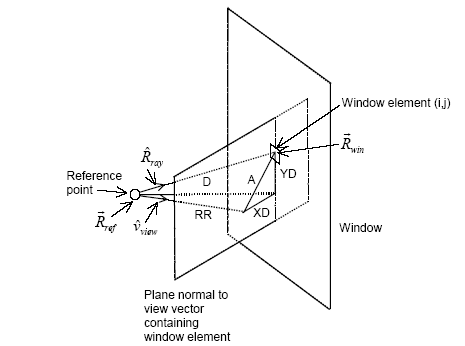
\includegraphics[width=0.9\textwidth, height=0.9\textheight, keepaspectratio=true]{media/image794.png}
\caption{Geometry for calculation of displacement ratios used in the glare formula. \protect \label{fig:geometry-for-calculation-of-displacement}}
\end{figure}

The factor \emph{p} can be obtained from graphs given in {[}Petherbridge \& Longmore, 1954{]} or it can be calculated from tabulated values of \emph{p\(_{H}\)}, the Hopkinson position factor {[}Hopkinson, 1966{]}, since \(p = p_H^{1.25}\) . The values resulting from the latter approach are given in Table~\ref{table:position-factor-for-glare-calculation}. Interpolation of this table is used in EnergyPlus to evaluate \emph{p} at intermediate values of \emph{x\(_{R}\)} and \emph{y\(_{R}\)}.

% table 26
\begin{longtable}[c]{|p{1.0in}p{0.4in}|p{0.4in}p{0.4in}p{0.4in}p{0.4in}p{0.4in}p{0.4in}p{0.4in}p{0.4in}|}
\caption{Position factor for glare calculation \label{table:position-factor-for-glare-calculation}}\\
\hline
            &      &\multicolumn{8}{c}{$x_R$: Horizontal Displacement Factor} \\
            &      & \textbf{0}     & \textbf{0.5}   & \textbf{1.0}   & \textbf{1.5}   & \textbf{2.0}   & \textbf{2.5}   & \textbf{3.0}   & \textbf{>3.0} \\
\hline
\textbf{$y_R$:}      & \textbf{0}    & 1.00  & 0.492 & 0.226 & 0.128 & 0.081 & 0.061 & 0.057 & 0 \\
\textbf{Vertical}    & \textbf{0.5}  & 0.123 & 0.119 & 0.065 & 0.043 & 0.029 & 0.026 & 0.023 & 0 \\
\textbf{Displacement}  & \textbf{1.0}  & 0.019 & 0.026 & 0.019 & 0.016 & 0.014 & 0.011 & 0.011 & 0 \\
\textbf{Factor}      & \textbf{1.5}  & 0.008 & 0.008 & 0.008 & 0.008 & 0.008 & 0.006 & 0.006 & 0 \\
            & \textbf{2.0}  & 0     & 0     & 0.003 & 0.003 & 0.003 & 0.003 & 0.003 & 0 \\
            & \textbf{>2.0} & 0     & 0     & 0     & 0     & 0     & 0     & 0     & 0 \\
\hline
\end{longtable}

The background luminance is:

\begin{equation}
{L_b} = {E_b}{\rho_b}
\end{equation}

where \emph{$\rho$\(_{b}\)} is approximated by the average interior surface reflectance of the entire room and

\begin{equation}
{E_b} = \max ({E_r},{E_s})
\end{equation}

where \emph{E\(_{r}\)} is the total internally-reflected component of daylight illuminance produced by all the windows in the room and \emph{E\(_{s}\)} is the illuminance setpoint at the reference point at which glare is being calculated. A precise calculation of \emph{E\(_{b}\)} is not required since the glare index (see next section) is logarithmic. A factor of two variation in \emph{E\(_{b}\)} generally produces a change of only 0.5 to 1.0 in the glare index.

\subsubsection{Glare Index}\label{glare-index}

The net daylight glare at a reference point due to all of the windows in a room is expressed in terms of a \emph{glare index} given by

\begin{equation}
{G_I} = 10{\log_{10}}\sum\limits_{i = 1}^{\scriptstyle \substack{number~of \\ windows}} {{{\rm{G}}_{\rm{i}}}}
\end{equation}

where \emph{G\(_{i}\)} is the glare constant at the reference point due to the \emph{i\(^{th}\)} window.
